% 'draft' mode can be used to speed up compilation
% \documentclass[13pt,a4paper,oneside]{hcmut-report}
\documentclass{latex/hcmut-report}

\usepackage{codespace}

% Draft watermark
% https://github.com/callegar/LaTeX-draftwatermark

% Encodings
\usepackage{gensymb,textcomp}

% Better tables
% Wide tables go to https://tex.stackexchange.com/q/332902
\usepackage{array,longtable,multicol,multirow,siunitx,tabularx}

% Better enum
\usepackage{enumitem}

% Graphics
\usepackage{caption,float}


% Add options for figures, like max width, framing, etc.
\usepackage[export]{adjustbox}

\usepackage{graphicx}

% References
% Use \Cref{} instead of \ref{}
\usepackage[nameinlink]{cleveref}

% FOR DEMONSTRATION PURPOSES, REMOVE IN PRODUCTION
\usepackage{float}
\usepackage{mwe}
\usepackage{longtable}
\usepackage{soul}
\usepackage{multicol}
\usepackage{tabularx, caption}
\usepackage{multirow}
\usepackage{tikz} 
\setlength{\parskip}{0.25em}
% Sub-preambles
% https://github.com/MartinScharrer/standalone

% Configurations
\coursename{Đồ án tổng hợp - hướng kỹ thuật dữ liệu (CO3127)}
\reporttype{ } 
\title{Report title h}
\advisor{ Dương Huỳnh Anh Đức }
\stuname{%
\hline
\textbf{Họ tên SV} & \textbf{MSSV} & \textbf{Nhóm - Lớp} \\
\hline
 Nguyễn Minh Nhựt & 2312550 & 2 - L02  \\
\hline
 Phạm Đình Phương Nam & 2312186 & 2 - L02  \\
\hline
 Đoàn Mạnh Tất  & 2313074  & 2 - L02  \\
\hline
 Phạm Đức Hoài Nam & 2212157 & 2 - L02  \\

\hline
} 


% Allow page breaks inside align* environment
%\allowdisplaybreaks{}

% Makes a lot of things blue, avoid at all costs
%\everymath{\color{blue}}

% Set depth of numbering for counters
\AtBeginDocument{\counterwithin{lstlisting}{section}}

% Rename some sections
%\AtBeginDocument{\renewcommand*{\contentsname}{Contents}}
%\AtBeginDocument{\renewcommand*{\refname}{References}}
%\AtBeginDocument{\renewcommand*{\bibname}{References}}

% Custom commands
%\newcommand*\mean[1]{\bar{#1}}

\begin{document}

\coverpage

\section*{Danh sách phân công công việc}
\begin{center}
\textbf{Nhóm: 2} 

  \begin{tabular}{|c|c|c|c|}
    \hline
    \textbf{STT} & \textbf{Họ và tên} & \textbf{Nhiệm vụ} & \textbf{Tỉ lệ hoàn thành} \\
    \hline
    1 & Nguyễn Minh Nhựt  &  & 100\% \\  \hline
    2 & Phạm Đình Phương Nam &  & 100\% \\     \hline
    3 & Đoàn Mạnh Tất &   & 100\% \\       \hline
    4 & Phạm Đức Hoài Nam &   & 100\% \\ \hline 
  \end{tabular}
\end{center}

\section*{Nhận xét từ giảng viên}
\begin{center}
  \begin{tabular}{|c|c|c|c|}
    \hline
    \textbf{STT} & \textbf{Họ và tên} & \textbf{Điểm số} & \textbf{Nhận xét} \\
    \hline
    1 &  Nguyễn Minh Nhựt   & \hspace{1cm} & \hspace{7.5cm} \\    \hline
    2 & Phạm Đình Phương Nam &  &  \\     \hline
    3 & Đoàn Mạnh Tất  &  &  \\       \hline
    4 & Phạm Đức Hoài Nam  &  &  \\ \hline 

  \end{tabular}
\end{center}

\clearpage
\pagenumbering{gobble}
\tableofcontents
%\listoffigures
%\listoftables
%\lstlistoflistings{}
\clearpage
\pagenumbering{arabic}
\setcounter{page}{1}

\setcounter{section}{0}

\section{ Giới thiệu}
\subsection{Tổng quan về Spotify }
Spotify là nền tảng phát nhạc trực tuyến hàng đầu thế giới, cung cấp dịch vụ nghe nhạc, podcast và audiobook theo yêu cầu cho hàng trăm triệu người dùng trên toàn cầu. Được ra mắt lần đầu tiên vào năm 2008 tại Thụy Điển, Spotify ra đời với mục tiêu tạo ra một giải pháp hợp pháp, tiện lợi và chống lại tình trạng vi phạm bản quyền âm nhạc trong thời kỳ bùng nổ Internet. Từ đó, Spotify đã nhanh chóng phát triển, trở thành biểu tượng cho sự thay đổi cách con người tiếp cận và thưởng thức âm nhạc.\\

Spotify hoạt động trên nhiều nền tảng như máy tính, điện thoại thông minh, TV, và các thiết bị IoT. Ứng dụng này hiện có mặt tại hơn 180 quốc gia và vùng lãnh thổ, sở hữu hơn 100 triệu bài hát cùng hơn 5 triệu podcast. Với hơn 600 triệu người dùng hàng tháng, trong đó hơn 240 triệu thuê bao trả phí, Spotify giữ vị trí dẫn đầu trong ngành công nghiệp phát nhạc trực tuyến toàn cầu.\\

\begin{figure}[h] % môi trường figure để quản lý hình
    \centering % căn giữa
    
\includegraphics[width=0.5\textwidth]{graphics/spotify_logo.png} % tên file hình
    \caption{Logo Spotify} % chú thích
    \label{fig:example} % nhãn để tham chiếu
\end{figure}

Không chỉ là một nền tảng âm nhạc, Spotify còn mang theo những giá trị mới mẻ về cá nhân hóa trải nghiệm. Hệ thống đề xuất thông minh dựa trên trí tuệ nhân tạo và dữ liệu lớn mang đến cho người dùng những playlist riêng biệt như Discover Weekly hay Release Radar. Qua đó, Spotify không chỉ thỏa mãn nhu cầu giải trí mà còn kết nối nghệ sĩ với khán giả, mở rộng ảnh hưởng văn hóa và hỗ trợ sự phát triển của ngành công nghiệp âm nhạc.\\

Một trong những nét đặc trưng nổi bật của Spotify là các chiến dịch sáng tạo và biểu tượng văn hóa số. Ví dụ, Spotify Wrapped – bản tổng kết hằng năm – đã trở thành hiện tượng toàn cầu, nơi hàng triệu người chia sẻ thói quen nghe nhạc của mình trên mạng xã hội. Bên cạnh đó, Spotify cũng chú trọng vào trải nghiệm đồng bộ qua Spotify Connect, cho phép người dùng dễ dàng phát nhạc trên nhiều thiết bị cùng lúc.\\
\begin{figure}[h] % môi trường figure để quản lý hình
    \centering % căn giữa
    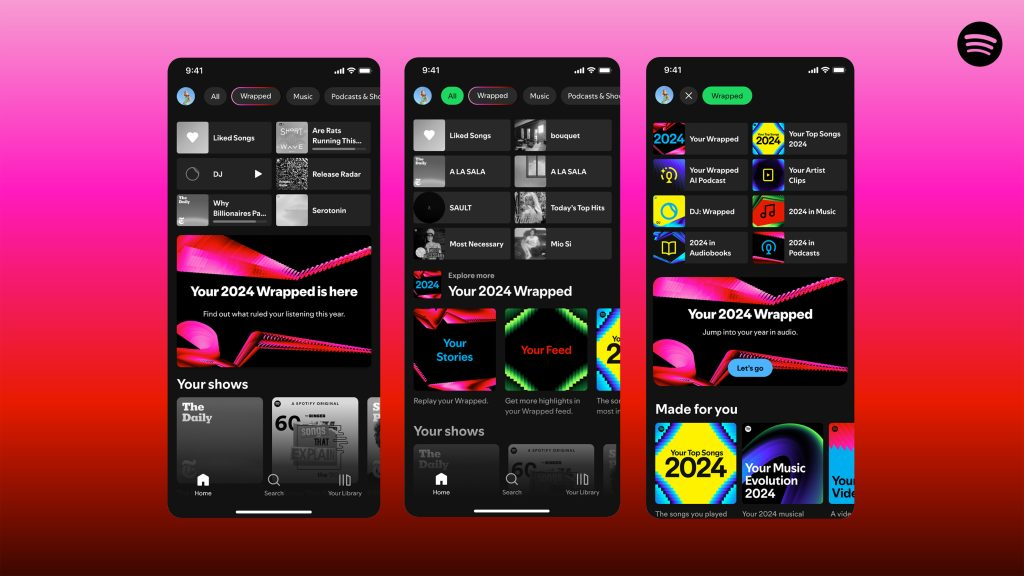
\includegraphics[width=0.5\textwidth]{graphics/spotify_wrapped.png} % tên file hình
    \caption{Logo Spotify} % chú thích
    \label{fig:example} % nhãn để tham chiếu
\end{figure}

Trong suốt quá trình phát triển, Spotify đã chứng kiến và góp phần tạo nên nhiều dấu ấn lịch sử của ngành nhạc số, thay đổi thói quen thưởng thức âm nhạc của cả một thế hệ. Không chỉ là nơi phát nhạc, Spotify còn là một nền tảng truyền cảm hứng, đưa âm nhạc đến gần hơn với cuộc sống hằng ngày và khẳng định sức mạnh của công nghệ trong việc kết nối con người qua âm nhạc.\\
\subsection{Vấn đề thực tế – Nhu cầu phân tích dữ liệu Spotify (xu hướng âm nhạc, gợi ý nhạc, phân tích nghệ sĩ)}
Trong kỷ nguyên số, lượng dữ liệu âm nhạc mà Spotify quản lý và tạo ra mỗi ngày là vô cùng khổng lồ: hàng tỷ lượt nghe, tìm kiếm, thêm vào playlist, chia sẻ và tương tác xã hội. Việc phân tích dữ liệu từ Spotify không chỉ phục vụ mục tiêu thương mại mà còn mang lại nhiều giá trị trong nghiên cứu, phát triển công nghệ và thậm chí là lĩnh vực văn hóa – xã hội. Một số nhóm đối tượng tiêu biểu có nhu cầu sử dụng dữ liệu này như sau:\\
\subsubsection{Nhà nghiên cứu âm nhạc và dữ liệu}
\begin{itemize}
    \item Phân tích xu hướng nghe nhạc theo thời gian, theo khu vực địa lý hoặc theo độ tuổi.

    \item Nghiên cứu mối liên hệ giữa đặc điểm âm nhạc (tempo, energy, danceability) với mức độ phổ biến.

    \item Tạo ra các mô hình dự đoán bài hát/ nghệ sĩ có khả năng trở thành xu hướng trong tương lai.
\end{itemize}
\subsubsection{Nhà nghiên cứu âm nhạc và dữ liệu}
\begin{itemize}
    \item Khám phá thói quen nghe nhạc cá nhân và so sánh với bạn bè hoặc cộng đồng.

    \item Tìm kiếm và gợi ý playlist phù hợp với tâm trạng, bối cảnh, hoạt động hàng ngày.
    
    \item Theo dõi các bảng xếp hạng như Top 50 Global hay Top 50 theo quốc gia để nắm bắt trào lưu âm nhạc mới.
\end{itemize}

\subsubsection{Nghệ sĩ và hãng thu âm}
\begin{itemize}
    \item Phân tích dữ liệu lượt nghe để đánh giá mức độ thành công của ca khúc, album hay tour diễn.

    \item Nghiên cứu thị trường mục tiêu: quốc gia, độ tuổi, giới tính của người nghe.

    \item Tối ưu hóa chiến lược phát hành (ngày ra mắt, thể loại, hợp tác nghệ sĩ) nhằm tối đa hóa doanh thu và mức độ lan tỏa.
\end{itemize}

\subsubsection{Doanh nghiệp và tổ chức quảng cáo}
\begin{itemize}
    \item Sử dụng dữ liệu hành vi người dùng để tối ưu hóa việc phân phối quảng cáo âm thanh và banner.

    \item Xác định nhóm khách hàng tiềm năng thông qua sở thích âm nhạc, từ đó đưa ra chiến lược tiếp thị hiệu quả hơn.

    \item Tận dụng dữ liệu thời gian thực để phân tích hiệu quả chiến dịch marketing (ví dụ: chiến dịch gắn liền với sự kiện âm nhạc quốc tế).
\end{itemize}

\subsubsection{Kỹ sư dữ liệu và nhà phát triển hệ thống}
\begin{itemize}
    \item Nhu cầu xử lý big data với tốc độ cao, từ đó yêu cầu hạ tầng dữ liệu mạnh mẽ (Apache Kafka, Spark, Hadoop).

    \item Đảm bảo tính chính xác, toàn vẹn và bảo mật của dữ liệu khi có hàng trăm triệu người dùng cùng truy cập.

    \item Xây dựng pipeline phân tích dữ liệu streaming theo thời gian thực, phục vụ cho hệ thống gợi ý cá nhân hóa.
\end{itemize}

\section{Mục tiêu đồ án}

\subsection{Thu thập và tiền xử lý dữ liệu}
\begin{itemize}
    \item Thu thập các dataset về Spotify từ Kaggle, API Sportify, ReccoBeats
    \item Làm sạch và chuẩn hóa dữ liệu: xử lý giá trị thiếu, định dạng ngày, chuẩn hóa các trường thuộc tính, loại bỏ dữ liệu dư thừa.
\end{itemize}

\subsection{Thiết kế và xây dựng hệ thống dữ liệu}
\begin{itemize}
    \item Thiết kế mô hình dữ liệu quan hệ (ERD, RM) dựa trên các file CSV đã chuẩn hóa.
    \item Tổ chức dữ liệu vào hệ quản trị CSDL (MySQL,..) nhằm đảm bảo tính toàn vẹn, tối ưu truy vấn và dễ dàng mở rộng.
    \item Áp dụng các kỹ thuật Data Engineering: indexing, trigger, backup/restore, tối ưu hóa dữ liệu.
\end{itemize}

\subsection{Xây dựng pipeline xử lý và phân tích dữ liệu}
\begin{itemize}
    \item Thiết kế mô hình dữ liệu quan hệ (ERD) dựa trên các file CSV đã chuẩn hóa.
    \item Tổ chức dữ liệu vào hệ quản trị CSDL (MySQL,..) nhằm đảm bảo tính toàn vẹn, tối ưu truy vấn và dễ dàng mở rộng.
    \item Áp dụng các kỹ thuật Data Engineering: indexing, trigger, backup/restore, tối ưu hóa dữ liệu.
\end{itemize}


\subsection{Phân tích và trực quan hóa dữ liệu Spotify}
\begin{itemize}
    \item Phân tích xu hướng âm nhạc: sự nổi bật của ca khúc/nghệ sĩ, vòng đời của bài hát (Hot/Cold cycle), sự khác biệt giữa các quốc gia.
    \item Khai thác đặc trưng âm nhạc (danceability, energy, acousticness, valence, tempo, v.v.) để tìm mối liên hệ với độ phổ biến.
    \item Trực quan hóa dữ liệu qua dashboard (Streamlit/Matplotlib/Seaborn), cho phép người dùng tra cứu bảng xếp hạng, so sánh quốc gia, xem biểu đồ xu hướng.
    \item còn tìm hiểu để thay đổi hoặc mở rộng
\end{itemize}

\subsection{Ứng dụng và mở rộng}
\begin{itemize}
    \item Hỗ trợ người dùng (sinh viên, nhà nghiên cứu, nghệ sĩ, doanh nghiệp) trong việc khai thác thông tin từ dữ liệu Spotify.
    \item Đề xuất khả năng mở rộng với Machine Learning như gợi ý bài hát, dự đoán bài hát tiềm năng sẽ vào bảng xếp hạng.
    \item Nâng cấp hệ thống thành mô hình phân tích dữ liệu streaming thời gian thực (Kafka + Spark) để phục vụ cập nhật liên tục.
    \item còn tìm hiểu để thay đổi hoặc mở rộng ( chọn 1 hướng để phát triển)
\end{itemize}






\section{Ràng buộc}

\subsection{Chuẩn hóa dữ liệu}
Áp dụng 1NF, 2NF, 3NF, BCNF

Thiết kế bảng: Track, Artist, Album, Playlist, User, Feature, Country/Chart

Giải thích phụ thuộc hàm, tách bảng

\section{Mô hình dữ liệu}
\subsection{ERD (Entity–Relationship Diagram)}
\subsection{Mô tả thực thể và thuộc tính (Track, Artist, Album, Feature, User, Playlist, Country)}
\subection{Mô hình dữ liệu quan hệ (các bảng, PK, FK, mô tả quan hệ n-n)}

\section{Ràng buộc}
\subsection{Ràng buộc về khóa}
\subsection{Ràng buộc dữ liệu (ví dụ: explicit chỉ nhận 0/1, popularity từ 0–100, duration_ms > 0)}

\section{Xử lý dữ liệu}
\subsection{Công nghệ xử lý (Python, Pandas, NumPy, Spotipy, SQLAlchemy, …)}
\subsection{Quy trình xử lý}

\section{Kiến trúc hệ thống}
Pipeline xử lý dữ liệu: thu thập → chuẩn hóa → lưu trữ → trực quan hóa/ML

Công nghệ: API Spotify + Python ETL + Database + Visualization (Tableau/Matplotlib/Seaborn/PowerBI)

Sơ đồ kiến trúc

\section{Hiện thực cơ sở dữ liệu}
\subsection{Tạo bảng và ràng buộc}
\subsection{Thêm dữ liệu từ dataset vào DB}
\subsection{Kết quả sau khi import}

\section{Nâng cao hiệu năng và tính nhất quán}
\subsection{Trigger (VD: khi thêm bài hát mới thì tự động cập nhật số lượng track trong album)}
\subsection{Index tối ưu (index cho track_id, artist_id, popularity, country)}

\section{Trực quan hóa và Phân tích}
\subsection{Trực quan hóa dữ liệu (biểu đồ top artists, top tracks theo quốc gia, phân tích audio features)
}

\subsection{Phân tích thống kê (phân bố tempo, danceability, energy theo genre)}

\subsection{So sánh theo thời gian (xu hướng nghe nhạc theo năm/tháng)}

\section{Ứng dụng Machine Learning}
\subsection{Bài toán lựa chọn (gợi ý nhạc / phân loại mood nhạc / dự đoán độ phổ biến)}
\subsection{Chuẩn bị dữ liệu (feature engineering)}
\subsection{Mô hình ML (Decision Tree, Random Forest, hoặc Neural Network đơn giản)}
\subsection{Đánh giá kết quả (accuracy, F1-score, confusion matrix, …)}

\section{Hiện thực giao diện hệ thống (nếu có)}
Web app / dashboard demo

Các màn hình chính: search track, thống kê top 10, ML prediction

\section{Source code}
Link GitHub / Google Drive

Hướng dẫn chạy

\section{Kết luận và Hướng phát triển}
Đánh giá kết quả đạt được

Hạn chế (dữ liệu thiếu track_id, giới hạn API Spotify, …)

Hướng phát triển (kết nối real-time API, streaming pipeline với Kafka/Spark, ML nâng cao)

\section{Phụ lục}
Đoạn code quan trọng (ETL, API call, ML training)

Biểu đồ, dataset mẫu

Test case

\end{document}